\documentclass{article}
\usepackage{graphicx}
\usepackage{amsmath}
\usepackage{amsfonts} 
% or 
\usepackage{amssymb}

\usepackage{tikz}
\usepackage{pgfplots}
\usepgfplotslibrary{fillbetween}
\usetikzlibrary{patterns}

\pgfplotsset{compat = newest}
\usepackage{cancel}
\usepackage[margin=1in]{geometry}
\usepackage{siunitx}
\usetikzlibrary{snakes}
\usepackage{pgflibrarysnakes}
\usetikzlibrary{decorations}
\usetikzlibrary{angles,quotes}
\begin{document}

\section{Base Units}
There are 7 base SI base units and they are as follows:

\begin{center}
  \begin{tabular}{ | c | c | c | }
    \hline
    Name & Unit Name & Unit \\ \hline
    Time & Seconds & \si{s} \\ \hline
    Mass & Kilogram & \si{kg} \\ \hline
    Current & Ampere & \si{A} \\ \hline
    Temperature & Kelvin & \si{K} \\ \hline
    Amount of substance & Mole & \si{mol} \\ \hline
    Luminosity & Candela & \si{cd} \\
    \hline
  \end{tabular}
\end{center}

\subsection{Derived Units}
From the si base units, one can derive other units such as \si{ms^{-1}}.
We can show this with the following:
\begin{gather*}
	s = \frac{d}{t} \\
	s = \frac{\si{m}}{\si{s}} \\
	s = \si{ms^{-1}}
\end{gather*}
Another more complex example: 
\begin{gather*}
	E_k = \frac{1}{2}mv^2 \\
	E_k = \frac{1}{2}\si{kg} \left (\si{ms^{-1}} \right )^2 \\
	E_k = \frac{1}{2}\si{kgm^{2}s^{-2}} \\
	\text{We remove the constant as it adds nothing to the unit} \\
	E_k = \si{kgm^{2}s^{-2}} \\
	J = \si{kgm^{2}s^{-2}} \\
\end{gather*}

\subsection{Prefixes}
We use prefixes to units to shorten down the format and to make values more human readible. Each prefix
represents a power of ten ($10^n$). The below table shows the different prefixes:
\begin{center}
    \begin{tabular}{|l|l|l|l|l|l|}
    \hline
    \textbf{Symbol} & \textbf{Name} & \multicolumn{2}{c|}{\textbf{What it means}} & \multicolumn{2}{c|}{\textbf{How to convert}} \\ \hline
    \si{T}          & Terra         & $10^{12}$  & $1,000,000,000,000$    & $\uparrow \div 1000$ & $\downarrow \times 1000$ \\ \hline
    \si{G}          & Giga          & $10^{9}$   & $1,000,000,000$        & $\uparrow \div 1000$ & $\downarrow \times 1000$ \\ \hline
    \si{M}          & Mega          & $10^{6}$   & $1,000,000$            & $\uparrow \div 1000$ & $\downarrow \times 1000$ \\ \hline
    \si{k}          & Kilo          & $10^{3}$   & $1,000$                & $\uparrow \div 1000$ & $\downarrow \times 1000$ \\ \hline
                    &               & $10^{0}$   & $1$                    & $\uparrow \div 1000$ & $\downarrow \times 1000$ \\ \hline
    \si{m}          & Milli         & $10^{-3}$  & $0.001$                & $\uparrow \div 1000$ & $\downarrow \times 1000$ \\ \hline
    \si{\mu}        & Micro         & $10^{-6}$  & $0.000001$             & $\uparrow \div 1000$ & $\downarrow \times 1000$ \\ \hline
    \si{n}          & Nano          & $10^{-9}$  & $0.00000001$           & $\uparrow \div 1000$ & $\downarrow \times 1000$ \\ \hline
    \si{p}          & Pico          & $10^{-12}$ & $0.000000000001$       & $\uparrow \div 1000$ & $\downarrow \times 1000$ \\ \hline
    \end{tabular}
\end{center}
\break

\section{Uncertanty}

\subsection{Measuring devices}
The typical uncertanty of a mesuring implement such as a ruler is half a division. So, for a typical ruler it would be $0.5\si{mm}$.
However, often a ruler needs to be alighned at two ends. this means that the actual uncertatny would be $1\si{mm}$.

\subsection{Calculationg Uncertanty}
Uncertanty is calculated using the following:
\begin{equation}
	\text{uncertanty} = \frac{\text{error}}{\text{value}}
\end{equation}

\subsection{Combining Uncertanty}
When multiplying two values with a percentage uncertanty that uncertanty is summed together.
For example, if given a cube with dimensions $50 \pm 1\si{mm}$, we can calculate the uncertanty of the volume
as follows:
\begin{gather*}
	\text{Start by calculating percentage uncertanty for a single side}\\
	\frac{1}{50} = 2 \% \\
	\text{Then multiply the uncertanty by $3$ because we are doing $\left (50 \pm 1 \si{mm} \right )^3$} \\
	2\% \times 3 = 6 \% \\
\end{gather*}
\subsection{Practicle: Measuring Density with Uncertanty}

\begin{center}
  \begin{tabular}{ | c | c | c | }
    \hline
    Mass & Volume & Density \\
	\hline	
    $550.2\si{g} \pm 0.05\si{g} (\pm 0.00908\%)$ & $(49 \pm 1\si{mm}(\pm 5\%))$ & $11200 \pm 101\si{kgm^{-3}}(\pm 9.05 \%)$ \\
	& $\times (20 \pm 1 \si{mm}(\pm 2.04\%))$ & \\
	& $\times (50 \pm 1 \si{mm}(\pm 2 \%))$ & \\
	& $ = 49 \pm 4.42 \si{cm^3}(\pm 9.04 \%)$ & \\
    \hline
  \end{tabular}
\end{center}

\section{Experiment Techniques}

\subsection{Accuracy}
Accuracy is how close a result is to the actual value.

\subsection{precision}
Precision is how close repeated readings are to eachother.

\subsection{Resolution}
Resolution is the smallest step a measuring device can measure.
For example, a meter ruler has a resolution of $1\si{mm}$ and a micrometer has
a resolution of $0.01\si{mm}$.


\break

\section{Archimedes' Priciple}
Upthrust in fluid is equal to that of the fluid displaced.

\subsection{Application}
Archimedes principle can be used to predict the resultant force of an object partially or fully submerged in a liquid.

\subsubsection{Example}
Given a granite cube with dimensions of length $3\si{cm}$ submerged in \textbf{water} suspended from a newton meter, predict the value on
the newton meter.

\begin{center}
	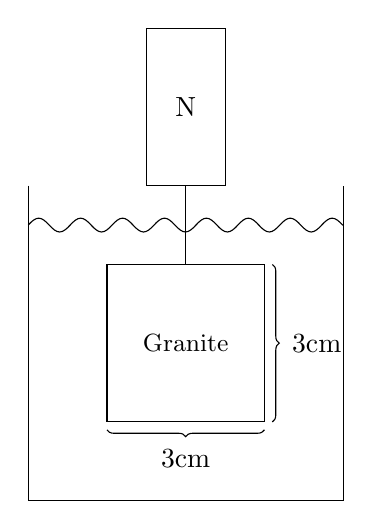
\begin{tikzpicture}
	\draw (-1,-1) rectangle (1,1);
	\draw (-0.5,2) rectangle (0.5,4);
	\draw (-2,2) -- (-2,-2) -- (2,-2) -- (2,2);
	\draw[snake=coil,segment aspect=0, line around snake=0, segment length=15.15] (-2,1.5) -- (2,1.5);
	\draw[] (0,2) -- (0,1);
	\node[] (n) at (0,3) {\si{N}};
	\node[] (m) at (0,0) {\small Granite};
	\node[label={[label distance=0.1]below:$3\si{cm}$}] (w) at (0,-1.1) {};
	\draw[snake=brace] (1,-1.1) -- (-1,-1.1);
	\draw[snake=brace] (1.1,1) -- (1.1,-1);
	\node[label={[label distance=0.1]right:$3\si{cm}$}] (w) at (1.1,0) {};
	\end{tikzpicture}
\end{center}

\begin{gather*}
	\text{Calculate the volume of the cube in \si{m^3}} \\
	0.03^3 = 0.000027 \si{m^3} \\
	\text{Calculate the mass of granite} \\
	0.000027 \si{m^3} \times \overbrace{2750\si{kgm^i{-3}}}^{\text{Density}} = 0.07425\si{kg} \\
	\text{Calculate the weight of granite} \\
	0.07425\si{kg} \times \overbrace{9.81\si{ms^{-2}}}^{\text{Feild Strength}} = 0.7839\si{N} \\
	\text{Volume of water displaced is the same as the volume of the cube because it is submerged}\\
	\text{Calculate the mass of water} \\
	0.000027\si{m^3} \times \overbrace{1000\si{kgm^{-3}}}^{\text{Density}} = 0.027\si{kg} \\
	\text{Calculate the upthrust} \\
	0.027\si{kg} \times \overbrace{9.81\si{ms^{-2}}}^{\text{Feild Strength}} = 0.26482\si{N} \\
	\text{Calculate the resultant force} \\
	0.72839 \si{N} - 0.26487 \si{N} = 0.464 \si{N} \\
\end{gather*}

\section{Laminar and Turbulant Flow}
\begin{itemize}
	\item Laminar -- Laminar flow is when
	\item Turbulant
\end{itemize}
We often assume laminar flow for simplicity.

\section{Stokes Law}
Stokes law states that the drag acting on a sphere in a
fluid is given by the following where $F_d$ is the drag
force, $\eta$ is the velocity of the fluid, $r$ is
the radius of the sphere and $v$ is the velocity of the sphere.
\begin{equation}
	F_d = 6\pi\eta rv
\end{equation}

\section{Vector and Scalar Quantities}
Vectors are values that hold both a magnitude and a direction whereas scalars only hold a magnitude.
\\\\
A non exaustive list of vector and scalar quantities:
\begin{center}
	\begin{tabular}{|l|l|}
		\hline
		\textbf{Scalar} & \textbf{Vector} \\ \hline
		Distance        & Displacement \\
		Speed           & Velocity \\
		Mass            & Force \\
		Energy          & Momentum \\
        Pressure        & Acceleration \\
		\hline
	\end{tabular}
\end{center}

\subsection{Resolving Vectors}
It is often useful for us to resolve vectors where we're given a magnitude and an angle into
their respective unit parts giving a value as a column vector or as two values, one horrizontal and
one vertical. We use triganometry to do this.
\\\\
The following shows how we can resolve a vector given a magnitude ($m$) and an angle ($\theta$):
\begin{center}
	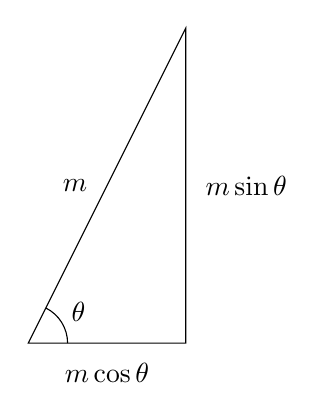
\begin{tikzpicture}
	\draw (-1,-2) coordinate (a) -- (1,-2) coordinate (b) -- (1,2) coordinate (c) -- cycle;

	\node[label={[label distance=0.1]left:$m$}] (w) at (0,0) {};

	\pic[draw,angle radius=.5cm,angle eccentricity=1.5,"$\theta$"] {angle= b--a--c};

	\node[label={[label distance=0.1]below:$m\cos\theta$}] (w) at (0,-2) {};
	\node[label={[label distance=0.1]right:$m\sin\theta$}] (w) at (1,0) {};

	\end{tikzpicture}
\end{center}

\subsection{Free Body Diagrams}
Free body diagrams are used to represent the forces acting on an object and their various directions,
they help with visualising problems.

\textbf{TODO}

\subsection{Extra Information}
For more information on vectors, such as addition, see maths notes.

\break

\section{Kinematics}
In kinematics we study the motion of bodies disregarding forces acting on it such as
air resistance.

\subsection{Definitions for Linear Motion}

\begin{center}
	\begin{tabular}{|l|l|}
		\hline
		\textbf{Quantity} & \textbf{Description} \\ \hline
		Displacement      & The distance traveled in a given direction and is the area under a velocity time graph. \\
		Instantanious Speed & Speed at any givent point in time; gradient of distance time graph. \\
		Average Speed & Rate of change of distance traveled. \\
		Velocity & Speed in a given direction (rate of change of displacement). \\
        Acceleration & Rate of change of velocity \\
		\hline
	\end{tabular}
\end{center}

\subsection{Distance vs Displacement}
Distance and displacement are different. Whereas distance is a scalar quantity, displacement is a vector quantity. Where
distance can represents the amount an object has moved displacement represents the amount an object has moved from a specific
starting point. This means that displacement can be affectively $0$ when distance is massive.

\subsection{SUVAT}
Suvat is a tool we can use to help with kinematics problems. 
\begin{itemize}
	\item $s$ -- Distance
	\item $u$ -- Initial Speed
	\item $v$ -- Final Speed
	\item $a$ -- Acceleration
	\item $t$ -- Time Interval	
\end{itemize}
We can substitute values next to each of the letters to work out which of the following formulae to use:
\begin{gather}
	v = at + u \\
	s = ut + \frac{1}{2}at^2 \\
	s = \left ( \frac{v + u}{2} \right )t \\
	v^2 = u^2 + 2as \\
	s = vt - \frac{1}{2}at^2 \\
\end{gather}
From there we can work out all of the other values in a question.

\subsubsection{Deriving SUVAT Euquations}

\begin{center}
	\begin{tikzpicture}
		\begin{axis}[
			axis lines=middle,
            xtick={0,2},
        	xticklabels={$0$,$t$},
			ytick={0,1,2},
			yticklabels={$0$,$u$,$v$},
			ymin=0,
		]

		\addplot[domain=0:4,range=0:4, name path=A] {x/2 + 1};
		\addplot[domain=0:4,range=0:4,dashed, name path=B] {1};
		\addplot[domain=0:4,range=0:4,dashed, name path=C] {2};
		\addplot[mark=none, dashed] coordinates {(2, 0) (2, 3)};

		\end{axis}
	\end{tikzpicture}

\end{center}
For the first equation we start by workinng out the gradient of the line.
And, as we know from previously, the gradient of velocity time graph
is acceleration.

\begin{gather}
	\frac{dy}{dx} = \frac{v - u}{t} = a \\
	a = \frac{v - u}{t} \\
	at = v - u \\
	v = u + at
\end{gather}
\\
For the next one we are finding the are under the line which we know
from earlier, on a velocity time graph, is the distance. We use the
area of a trapesium for this.

\begin{gather}
	\left ( \frac{a + b}{2} \right ) h = \left ( \frac{v + u}{2} \right )t \\
	s = \left ( \frac{v + u}{2} \right )t \\
\end{gather}
\\
For the next equation we can substitute $v$ into our second formula
\begin{gather}
	s = \left ( \frac{v + u}{2} \right )t \\
	s = \left ( \frac{u + at + u}{2} \right )t = \left ( \frac{2u + at}{2} \right )t \\
	s = \left ( u + \frac{at}{2} \right )t = ut + \frac{1}{2}at^2 \\
\end{gather}
\\
For our next equation we can do the following
\begin{gather}
	v = at + u \\
	t = \frac{v - u}{a} \\
	s = \left ( \frac{v + u}{2} \right )t \\
	s = \left ( \frac{v + u}{2} \right )\left (\frac{v - u}{a}\right ) \\
	s = \frac{v^2 - u^2}{2a} \\
	2as = v^2 - u^2 \\
	v^2 = u^2 + 2as \\
\end{gather}
\\
For our final equation be can just rearrange a previous equation.

\begin{gather}
	u = v - at \\
	s = \left ( \frac{v + u}{2} \right )t \\
	s = \left ( \frac{v + v - at}{2} \right )t = \left ( \frac{2v - at}{2} \right )t \\
	s = \left ( v - \frac{at}{2} \right )t = vt - \frac{1}{2}at^2 \\
\end{gather}

\section{Elasticity}

Extension -- difference in length due to being stretched


\begin{equation}
	F = k\Delta x
\end{equation}

\begin{itemize}
	\item Force is a measure of stiffness
	\item gradient is measure of stiffness of the spring.
	\item Works for extension and compression.
	\item Hooks law works in the elastic region. up to the limit of proportionality.
	\item limit of proportionality is close to the elastic limit. it is the point in which the extension becomes plastic instead of elastic.
	\item this means that it's no longer linear.
	\item gradient of plastic line tends to be the same
	\item Adding two springs in series doubles the extension.
	\item Adding two springs in parallel halfs the extension.
\end{itemize}

\textbf{TODO: READING + Definitions}

\begin{itemize}
	\item \textbf{Stiffness} -- A stiff material exibits very small deformation even when subjected to large forces.
	\item \textbf{Toughness} -- Tough materials are able to absorb the energie from impacts and shocks without breaking.
	\item \textbf{Brittleness} -- Brittle materials will shatter or crack when subjected to force
	\item \textbf{Malleability} -- A malleable material can be hammered out into thin sheets.
	\item \textbf{Ductility} -- A ductile material can be drawn into wires
\end{itemize}


\section{Newtons Laws}

\subsection{Newtons First Law}
\begin{equation}
	\sum F = 0
\end{equation}
The body remains at rest at a state of uniform motion unless the forces acting on it are not in equlirium
\\\\
An object will stay still or carry on moving exactly the way it was unless unbalanced force acts on it.
\\\\
When there is no resultant force (it is at an equalibriumdc, the object remains stationary or at a constant velocity

\subsubsection{Inertia}
The property of a body to stay in a state of rest or uniform motion.
\\\\
The reluctance of a body to change its motion.
\\\\
Angry LHN has a greater inertia than calm LHN.
\\\\
Very linked to Newtons first law.

\subsection{Newtons Second Law}
\begin{equation}
	\sum F \ne 0
\end{equation}
When there is a resultant for the object accelerates, changes direction or deformation (change in structure).

\begin{equation}
	F = ma
\end{equation}
If an unbalanced force acts on an object then its velocity will change.
It will either change direction, speed up or slow down, and that includes stopping.

\subsection{Newtons Third Law}
Every action has an equal and oposite reaction \ldots \textbf{of the same type}.
\\\\
Compare the same forces, can't compare normal contact force and weight.
\\\\
When body A exerts a force on body B, an equal an oposite force \textbf{of the same type} is exerted by
body B on body A.
\\\\
Normal contact force is electrostatic force as you don't technically touch anything.

\section{Drag and Terminal Velocity}
Terminal velocity is reached when the following equation is true:
\begin{equation}
	F_d = F_w
\end{equation}

A force is a push, pull or twist. An interaction between two physical bodies with mass.
It can cause the physical bodies to undergo a change such as change in acceleractoin, direction or structure.
\\\\
Friction is resistance between two physical bodies
\\\\
Drag is resistance on a physical body as it moves through a fluid.


\section{Youngs Modulus}

\begin{gather}
	\sigma = \frac{F}{A}\\
	\epsilon = \frac{\Delta l}{l}\\
	E = \frac{\sigma}{\epsilon} = \frac{Fl}{A\Delta l}\\
	\Delta l = \frac{Fl}{AE}
\end{gather}


\subsection{Composite Wires}
For composite wires, calculate each wire seperately. Forces stay the same.

\subsection{Stress Strain Graphs}

The formula for the Hooke's law region is as follows: 
\begin{equation}
	\sigma = E \epsilon
\end{equation}
Stress strain graphs have the same properties as force extension graphs.

The ultimate tensile strength is when the material affectively breaks and will keep extending no matter the force. It is the
largest force that can be applied to that material.
It actually breaks at the breaking point.

Increasing Carbon content  in steel increases Youngs Modulus and thus the stiffness of the material. This inturn increases
the strength of the steel. However this also makes it morei brittle.

Plastics have a very large plastic region. Brittle plasics have a much smaller plastic region.

Copper has a large plastic region. 

Aluminionm alloys are stronger than copper and stiffer.

Glass has a very small plastic region.

\end{document}
